% Saved into the git report.tex at 2017/12/15 at 00:11 from this web
\documentclass{article}
\usepackage[utf8]{inputenc}
\usepackage{pythonhighlight}

\usepackage[utf8]{inputenc}
\usepackage{graphicx}
\graphicspath{ {fig/} }
\usepackage{listings}
\usepackage{color}
\usepackage{float}

% Use better tables
\usepackage{booktabs}

% Units
\usepackage{siunitx}

\usepackage{listings}

\title{Lab 6 - CSN: Network dynamics}
\author{Pierre-Antoine Porte \\ \texttt{porte.pierreantoine@gmail.com}
\and Rodrigo Arias Mallo \\ \texttt{rodarima@gmail.com}}
\date{\today}

%%% \def\arraystretch{1.5}

\begin{document}

\maketitle

\section{Introduction}

In this session, we had to model 3 different models following the dynamical
principles of the Barabasi-Albert model. Those principles are: vertex growth and
preferential attachment. The different models we needed to implements were the
following:

\begin{itemize}
	\item Barabasi-Albert with the dynamical principles
	\item Barabasi-Albert with random attachment instead of preferential
	attachment (only one dynamical principle).
	\item Barabasi-Albert with vertex growth suppressed (only one dynamical
	principle).
\end{itemize}

Those models were simulated and the data kept in files so we could analyze
mathematical properties of those models.

In this report we will show our results regarding those models and their
analysis. We will discuss those results and explain them. Then we will explain
how we implemented the model simulations and what we used to analyze it in the
Methods section.

\section{Results}

The columns represents the models where respectively:

\begin{itemize}
		\item A is Barabasi-Albert
		\item B is with random attachment instead of preferential
		\item C is without vertex growth
\end{itemize}

The tables in annexes (\ref{tab:AICdd} to \ref{tab:AICdt1000}) uses AIC to
measure $\delta$ between each model.

\begin{figure}[h]
    \centering
    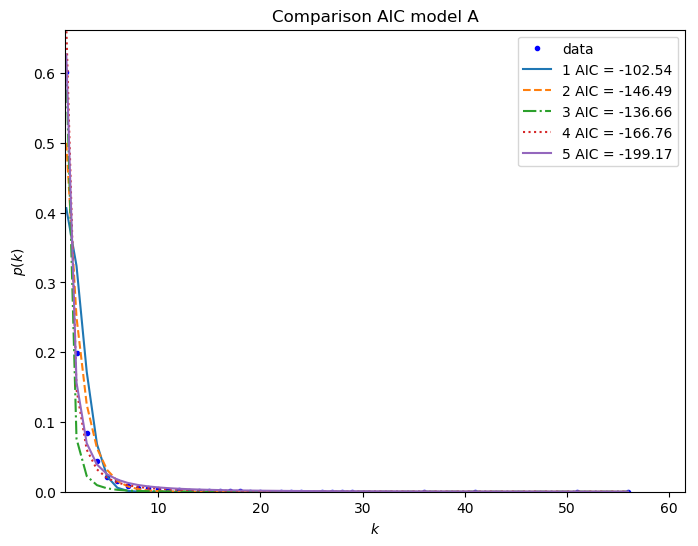
\includegraphics[width=0.5\textwidth]{modelA/all_dd.png}
    \caption{Distribution degree for model A}
    \label{fig:all_dd_A}
\end{figure}

\begin{figure}[h]
    \centering
    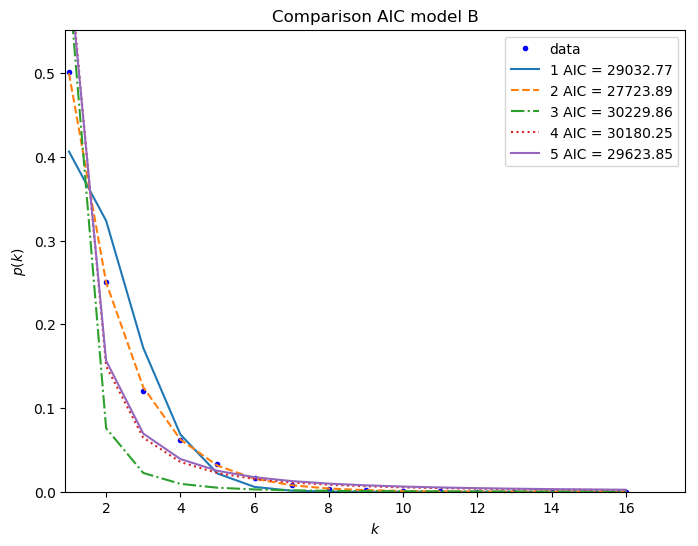
\includegraphics[width=0.5\textwidth]{modelB/all_dd.png}
    \caption{Distribution degree for model B}
    \label{fig:all_dd_B}
\end{figure}

\begin{figure}[h]
    \centering
    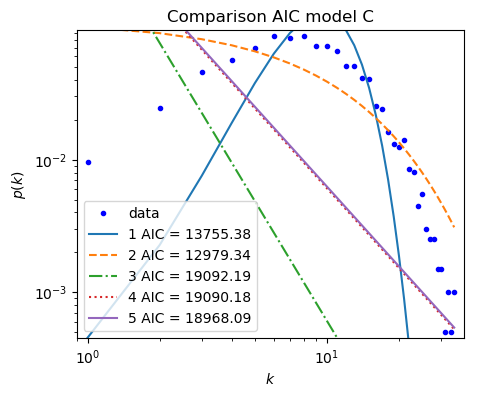
\includegraphics[width=0.5\textwidth]{modelC/all_dd.png}
    \caption{Distribution degree for model C}
    \label{fig:all_dd_C}
\end{figure}

% TODO: add dt1->1000 for each model

\section{Discussion}

\subsection{Simulation of the models}

As explained in section Methods, we used $m_0$ and $n_0$ always with the same
values (which can be however different for each model). We never compared the
models with different $m_0$ or $n_0$ for the same model. It could have indicate
us if the model behave differently given different graph in input. We could have
went further and do this but we preferred to focus on the analysis of our
different models with the input specified in the methods section.

\subsection{Barabasi-Albert}

% TODO Understand why we don't have this barabasi albert property %

\subsection{Vertex degree over time}

We checked if the power-law dependency with 1/2 exponent gives the best fit to
all the time series as required by the statement. This power-law dependency is
not the best fit. This power-law is model 1, which has an AIC higher than model
2 (see tables \ref{tab:AICdt1} to \ref{tab:AICdt1000}. In fact the best model is
model 2, defined as \textbf{$a*{t^b}$}, which is the exponential growth. It
makes sense because with one free parameter we can better optimize this model to
fit the data, by adapting b to somewhat close to 1/2 as expected in model 1.

However if we look at table \ref{tab:paramsdt1} to \ref{tab:paramsdt1000}, we
see that $b \approx 0.5$ only for $t_i = 1000$ (table \ref{tab:AICdt1000}).

\subsection{Degree distribution}

\subsection{Barabasi-Albert without preferential attachment}

\subsection{Vertex degree over time}

For table \ref{tab:AICdt1} to \ref{tab:AICdt1000}, best model is as suggested by
the statement the logarithmic model of the 4\textsuperscript{th} model. Indeed,
we have 0 as $\delta$AIC for the vertex degree over time for this model and for every
$t_i$ chosen to look at the vertex.

%todo add plot

\subsection{Degree distribution}


The best model for the degree distribution for the Barabasi Albert model without
preferential attachment is the geometric one (model 1). Actually only the
variant of the geometric model is good (model 1+), as we can see in table
\ref{tab:AICdd}. The model 1 has a $\delta$AIC too high. However by replacing
correctly the generated data from model 1, we now have a $\delta$AIC of 0.
Thus, the geometric model variant is the best model.

By looking at the figure \ref{fig:ADD THE PLOT}, we can clearly see that
the geometric model (orange one)
is a really good approximation of our data. It even goes through a lot of
points of the actual data point we have.

%todo add ref plot


\subsection{Barabasi-Albert without vertex growth}

\subsubsection{Vertex degree over time}

As expected by statement, this model's scaling vertex degree over time should
fit a linear scale. By computing the AIC and making the $\delta$ (see tables
\ref{tab:AICdt1} to \ref{tab:AICdt1000}) we have seen that the linear model
was good. Also, we are really confident by saying it's linear when we look at
the plot generated for model3, for every $t_is$. However we find that model0,
0+, 2 and 2+ are the best. Sometimes it's 0(+), sometimes it's 2(+). Model 2 is
represented as $at^b$, as b is close to 1 as we can see in tables
\ref{tab:AICdt1} to \ref{tab:AICdt1000}, which explain this good fit for model
2 and 2+.

\subsubsection{Degree distribution}

As stated by the statement, the degree distribution for this model should be
closer to a binomial distribution. Indeed it looks like it, but we found out it
looked even more of a displaced poisson with on a different scale. If we took
$\lambda = 2$, then we would have a fastly increasing and decreasing poisson
which is what we want. However, this Poisson has a mean of $\lambda = 2$.
Therefore, it does not fit our data which has a mean of approximately 10.
%TODO VERIFY the mean
So we displaced the poisson and adjusted the scale. The lasting problem was that
due do this scale and displacement, our model never produces data $\approx 0$
whereas the generated model data had a lot of values $\approx 0$.

In the end we chose to use a poisson distribution as we did in lab2. It's not a
really good fit but it's still the best fit we have. You can see this plot in
figure
%TODO ref figure

We also made sure that the distribution giving the best fit in not a power-law,
it's looking more of a Gausian one. However since it's not symetric it was hard
to model the data using a normal law, for example.

\section{Methods} \label{methods}

For the default \textit{Barabasi-Albert} and model with random attachment the
initial graph was an empty graph with only one vertex.

For the model without vertex growth, we used an unconnected graph with $t_max$
vertices. Because we have no vertex growth, the vertices are not increasing and
$n_0$ = $n_tmax$.

For the three models we used $m_0 = 0$ to used "\textit{clean}" and
"\textit{empty}" graphs.

We measured the growth of the vertex degree over time and the degree
distribution for each model. The vertex degree was measured over the time for
$t_i = 1, 10, 100, 1000, 10000$ successively.

We used python for generating the models, to store the results and to analyze
the data. For each BA model $M$ a folder in \texttt{data/model$M$/} contains all
the results produced from this model. Inside, the degree sequence is stored in
the file \texttt{dseq.txt}, the degree distribution in \texttt{dd.txt} and for
each $T$ in the arrival time, we produced \texttt{dt\_$t_i$.txt} tracing the
degree of the vertex arriving at time $t$.

\subsection{Generating model with preferential attachment}

While trying to define how to make the preferential attachment for model 3 we
faced a problem. We were choosing from the edges to be linked to our vertex in
an array of probability p, with the degree of the node over the sum of the
degrees of all nodes as:

\begin{python}
    p[i] = vertex.degree()/sum(graph.all_degrees())
\end{python}

However, with this, if you had m0 = 5 and only 4 vertices with a degree > 0,
then you could not choose your 5 vertices, and it did not work.

What we needed to do is counting stubs instead of degree, with a virtual stub
for each unconnected vertex. Therefore our array of probability p was computed
as:

\begin{python}
if vertex.degree == 0:
    p[i] = 1 / sum(graph.all_degrees()) + sum(number_of_nodes_with_degree_0)
else:
    p[i] = vertex.degree() / (sum(graph.all_degrees()) + sum(number_of_nodes_with_degree_0))
\end{python}

In the end the degree was represented with the number of stubs.


\section*{Annexes}

% AICs

\begin{table}[H]
	\centering
	\begin{tabular}{rrrr}
\toprule
     &        A &        B &        C \\
\midrule
   1 & \num{7245.741} & \num{1308.885} &  \num{776.040} \\
   2 & \num{1097.608} &    \num{0.000} &    \num{0.000} \\
   3 &  \num{606.012} & \num{2505.972} & \num{6112.841} \\
   4 &  \num{359.648} & \num{2456.367} & \num{6110.839} \\
   5 &    \num{0.000} & \num{1899.960} & \num{5988.746} \\
\bottomrule
\end{tabular}
	\caption{$\delta$ for the degree distribution.}
	\label{tab:AICdd}
\end{table}
\begin{table}[H]
	\centering
	\begin{tabular}{lrrr}
\toprule
     &         1 &         2 &         3 \\
\midrule
 0   & \num{69534.390} & \num{59969.865} & \num{10786.775} \\
 1   & \num{45188.426} & \num{48383.218} & \num{38204.833} \\
 2   &     \num{0.000} &  \num{4088.919} &    \num{33.872} \\
 3   & \num{57486.358} & \num{23686.609} & \num{65632.205} \\
 4   & \num{57130.622} &    \num{10.271} & \num{49999.142} \\
 0+  & \num{45767.062} & \num{22835.391} &  \num{4019.623} \\
 1+  & \num{27730.356} & \num{25665.773} & \num{26144.944} \\
 2+  & \num{19115.101} & \num{10442.574} &     \num{0.000} \\
 3+  &  $\infty$    &  $\infty$    &  $\infty$    \\
 4+  & \num{12117.889} &     \num{0.000} &  \num{9608.871} \\
\bottomrule
\end{tabular}
	\caption{$\delta$ for the vertex degree over time for $t_i = 1$.}
	\label{tab:AICdt1}
\end{table}
\begin{table}[H]
	\centering
	\begin{tabular}{lrrr}
\toprule
     &         1 &         2 &         3 \\
\midrule
 0   & \num{56219.491} & \num{56948.832} &  \num{3294.824} \\
 1   & \num{33958.147} & \num{44276.525} & \num{35679.447} \\
 2   &  \num{5638.288} &  \num{4262.024} &    \num{77.463} \\
 3   & \num{80808.086} & \num{75603.323} & \num{65467.831} \\
 4   & \num{41881.941} &  \num{5870.707} & \num{48564.528} \\
 0+  & \num{33417.747} & \num{22409.635} &  \num{1463.430} \\
 1+  & \num{17922.167} & \num{15043.736} & \num{23894.852} \\
 2+  & \num{11109.884} &  \num{9443.397} &     \num{0.000} \\
 3+  &  $\infty$    &  $\infty$    &  $\infty$    \\
 4+  &     \num{0.000} &     \num{0.000} &  \num{4786.908} \\
\bottomrule
\end{tabular}
	\caption{$\delta$ for the vertex degree over time for $t_i = 10$.}
	\label{tab:AICdt10}
\end{table}
\begin{table}[H]
	\centering
	\begin{tabular}{lrrr}
\toprule
     &         A &         B &         C \\
\midrule
 0   & \num{46992.180} & \num{56158.051} &  \num{6775.516} \\
 1   & \num{26745.892} & \num{40993.239} & \num{34445.263} \\
 2   &  \num{4084.008} & \num{11373.071} &  \num{1083.024} \\
 3   & \num{70608.550} & \num{76491.996} & \num{62248.713} \\
 4   & \num{30090.842} & \num{24884.091} & \num{46399.114} \\
 0+  & \num{22011.767} & \num{27947.947} &   \num{343.071} \\
 1+  & \num{10879.865} & \num{20065.047} & \num{20084.117} \\
 2+  &  \num{3419.044} & \num{14228.805} &     \num{0.000} \\
 3+  &  $\infty$    &  $\infty$    &  $\infty$    \\
 4+  &     \num{0.000} &     \num{0.000} &  \num{1983.962} \\
\bottomrule
\end{tabular}
	\caption{$\delta$ for the vertex degree over time for $t_i = 100$.}
	\label{tab:AICdt100}
\end{table}
\begin{table}[H]
	\centering
	\begin{tabular}{lrrr}
\toprule
     &         1 &         2 &         3 \\
\midrule
 0   & \num{24212.569} & \num{24852.123} & \num{16241.758} \\
 1   &  \num{8639.541} &  \num{4706.668} & \num{35197.595} \\
 2   &  \num{4130.729} &  \num{4019.593} &   \num{465.222} \\
 3   & \num{58036.196} & \num{55068.283} & \num{69970.214} \\
 4   & \num{31443.880} & \num{27424.662} & \num{49730.948} \\
 0+  &     \num{0.021} & \num{10189.872} &  \num{2862.488} \\
 1+  &  \num{5672.115} &  \num{3420.122} & \num{13800.604} \\
 2+  &     \num{0.000} &  \num{1158.596} &   \num{424.130} \\
 3+  &  $\infty$    &  $\infty$    &  $\infty$    \\
 4+  &   \num{159.748} &     \num{0.000} &     \num{0.000} \\
\bottomrule
\end{tabular}
	\caption{$\delta$ for the vertex degree over time for $t_i = 1000$.}
	\label{tab:AICdt1000}
\end{table}

% Params
\begin{table}[H]
	\centering
	\begin{tabular}{lrrr}
\toprule
 Dataset        &      1 &      2 &      3 \\
\midrule
 $1_{\lambda}$  &  \num{1.593} &  \num{1.593} & \num{10.000} \\
 $2_{q}$        &  \num{0.500} &  \num{0.500} &  \num{0.100} \\
 $4_{\gamma}$   &  \num{2.189} &  \num{2.078} &  \num{2.000} \\
 $5_{\gamma}$   &  \num{2.000} &  \num{2.000} &  \num{2.000} \\
 $5_{k_{\max}}$ & \num{20.000} & \num{20.000} & \num{20.000} \\
\bottomrule
\end{tabular}
	\caption{Parameters for degree distribution models fitting.}
	\label{tab:param_dd}
\end{table}
\begin{table}[H]
	\centering
	\begin{tabular}{lrrr}
\toprule
 Dataset   &       A &       B &         C \\
\midrule
 $0 a$     &   \num{0.005} &   \num{0.002} &     \num{0.001} \\
 $1 a$     &   \num{0.434} &   \num{0.134} &     \num{0.110} \\
 $2 a$     &   \num{1.616} &   \num{3.348} &     \num{0.000} \\
 $2 b$     &   \num{0.350} &   \num{0.133} &     \num{1.166} \\
 $3 a$     &  \num{14.000} &   \num{8.637} &    \num{-0.000} \\
 $3 c$     &   \num{0.000} &   \num{0.000} &    \num{-0.527} \\
 $4 a$     &   \num{3.792} &   \num{1.222} &     \num{0.837} \\
 $4 d_1$   &  \num{-0.849} &   \num{1.117} &    \num{-0.871} \\
 $0+ a$    &   \num{0.003} &   \num{0.000} &     \num{0.002} \\
 $0+ d$    &  \num{14.000} &   \num{8.496} &    \num{-0.735} \\
 $1+ a$    &   \num{0.370} &   \num{0.072} &     \num{0.178} \\
 $1+ d$    &   \num{5.000} &   \num{5.000} &    \num{-5.000} \\
 $2+ a$    &   \num{0.500} &   \num{0.413} &     \num{0.000} \\
 $2+ b$    &   \num{0.466} &   \num{0.300} &     \num{1.155} \\
 $2+ d$    &   \num{5.000} &   \num{5.000} &    \num{-0.058} \\
 $3+ a$    &   \num{0.289} &   \num{0.289} &     \num{0.289} \\
 $3+ c$    &   \num{0.853} &   \num{0.853} &     \num{0.853} \\
 $3+ d$    & \num{-10.000} & \num{-10.000} &   \num{-10.000} \\
 $4+ a$    &  \num{12.971} &   \num{1.230} &    \num{48.860} \\
 $4+ d_1$  & \num{952.161} &   \num{1.413} & \num{27177.319} \\
 $4+ d_2$  & \num{-80.698} &  \num{-0.060} &  \num{-500.000} \\
\bottomrule
\end{tabular}
	\caption{Parameters for the vertex degree over time for $t_i = 1$.}
	\label{tab:paramsdt1}
\end{table}
\begin{table}[H]
	\centering
	\begin{tabular}{lrrr}
\toprule
 Param        &       A &       B &       C \\
\midrule
 $T0$, $a$    &   \num{0.003} &   \num{0.001} &   \num{0.001} \\
 $T1$, $a$    &   \num{0.237} &   \num{0.093} &   \num{0.087} \\
 $T2$, $a$    &   \num{1.036} &   \num{1.795} &   \num{0.001} \\
 $T2$, $b$    &   \num{0.330} &   \num{0.159} &   \num{1.070} \\
 $T3$, $a$    &  \num{-0.330} &  \num{-0.331} &  \num{-0.352} \\
 $T3$, $c$    &  \num{-1.363} &  \num{-1.363} &  \num{-0.566} \\
 $T4$, $a$    &   \num{2.079} &   \num{0.820} &   \num{0.693} \\
 $T4$, $d_1$  &  \num{-9.843} &  \num{-9.408} &  \num{-9.875} \\
 $T0+$, $a$   &   \num{0.001} &   \num{0.000} &   \num{0.001} \\
 $T0+$, $d$   &  \num{10.366} &   \num{5.424} &  \num{-0.220} \\
 $T1+$, $a$   &   \num{0.172} &   \num{0.036} &   \num{0.139} \\
 $T1+$, $d$   &   \num{4.885} &   \num{4.303} &  \num{-3.958} \\
 $T2+$, $a$   &   \num{0.800} &   \num{0.314} &   \num{0.000} \\
 $T2+$, $b$   &   \num{0.355} &   \num{0.300} &   \num{1.088} \\
 $T2+$, $d$   &   \num{0.798} &   \num{2.893} &   \num{0.076} \\
 $T3+$, $a$   &   \num{0.289} &   \num{0.289} &   \num{0.289} \\
 $T3+$, $c$   &   \num{0.853} &   \num{0.853} &   \num{0.853} \\
 $T3+$, $d$   & \num{-10.000} & \num{-10.000} & \num{-10.000} \\
 $T4+$, $a$   &   \num{3.238} &   \num{0.970} &   \num{1.874} \\
 $T4+$, $d_1$ &  \num{-8.242} &  \num{-1.528} &  \num{11.972} \\
 $T4+$, $d_2$ & \num{-10.000} &  \num{-1.258} & \num{-10.000} \\
\bottomrule
\end{tabular}
	\caption{Parameters for the vertex degree over time for $t_i = 10$.}
	\label{tab:paramsdt10}
\end{table}
\begin{table}[H]
	\centering
	\begin{tabular}{lrrr}
\toprule
 Param        &       A &       B &       C \\
\midrule
 $T0$, $a$    &   \num{0.001} &   \num{0.001} &   \num{0.001} \\
 $T1$, $a$    &   \num{0.083} &   \num{0.064} &   \num{0.074} \\
 $T2$, $a$    &   \num{0.422} &   \num{0.735} &   \num{0.000} \\
 $T2$, $b$    &   \num{0.313} &   \num{0.220} &   \num{1.122} \\
 $T3$, $a$    &  \num{-0.500} &  \num{-0.500} &  \num{-0.500} \\
 $T3$, $c$    &  \num{-0.500} &  \num{-0.500} &  \num{-0.500} \\
 $T4$, $a$    &   \num{0.718} &   \num{0.563} &   \num{0.568} \\
 $T4$, $d_1$  & \num{-15.000} & \num{-15.000} & \num{-15.000} \\
 $T0+$, $a$   &   \num{0.000} &   \num{0.000} &   \num{0.001} \\
 $T0+$, $d$   &   \num{3.674} &   \num{3.410} &  \num{-0.463} \\
 $T1+$, $a$   &   \num{0.059} &   \num{0.033} &   \num{0.128} \\
 $T1+$, $d$   &   \num{1.864} &   \num{2.366} &  \num{-4.056} \\
 $T2+$, $a$   &   \num{0.498} &   \num{0.289} &   \num{0.001} \\
 $T2+$, $b$   &   \num{0.300} &   \num{0.300} &   \num{1.047} \\
 $T2+$, $d$   &  \num{-0.328} &   \num{1.054} &  \num{-0.304} \\
 $T3+$, $a$   &   \num{0.289} &   \num{0.289} &   \num{0.289} \\
 $T3+$, $c$   &   \num{0.853} &   \num{0.853} &   \num{0.853} \\
 $T3+$, $d$   & \num{-10.000} & \num{-10.000} & \num{-10.000} \\
 $T4+$, $a$   &   \num{1.614} &   \num{0.931} &   \num{1.757} \\
 $T4+$, $d_1$ &  \num{50.000} & \num{-10.000} & \num{-10.000} \\
 $T4+$, $d_2$ &  \num{-7.569} &  \num{-3.089} & \num{-10.000} \\
\bottomrule
\end{tabular}
	\caption{Parameters for the vertex degree over time for $t_i = 100$.}
	\label{tab:paramsdt100}
\end{table}
\begin{table}[H]
	\centering
	\begin{tabular}{lrrr}
\toprule
 Dataset   &         A &       B &         C \\
\midrule
 $0 a$     &     \num{0.000} &   \num{0.000} &     \num{0.001} \\
 $1 a$     &     \num{0.036} &   \num{0.034} &     \num{0.120} \\
 $2 a$     &     \num{0.016} &   \num{0.025} &     \num{0.005} \\
 $2 b$     &     \num{0.596} &   \num{0.537} &     \num{0.864} \\
 $3 a$     &    \num{-0.500} &  \num{-0.500} &    \num{-0.500} \\
 $3 c$     &    \num{-0.500} &  \num{-0.500} &    \num{-0.500} \\
 $4 a$     &     \num{0.306} &   \num{0.300} &     \num{1.013} \\
 $4 d_1$   &   \num{-15.000} & \num{-15.000} &   \num{-15.000} \\
 $0+ a$    &     \num{0.000} &   \num{0.000} &     \num{0.001} \\
 $0+ d$    &     \num{0.925} &   \num{1.003} &     \num{0.928} \\
 $1+ a$    &     \num{0.041} &   \num{0.037} &     \num{0.183} \\
 $1+ d$    &    \num{-0.360} &  \num{-0.224} &    \num{-4.921} \\
 $2+ a$    &     \num{0.000} &   \num{0.334} &     \num{0.004} \\
 $2+ b$    &     \num{1.001} &   \num{0.300} &     \num{0.880} \\
 $2+ d$    &     \num{0.926} &  \num{-1.835} &     \num{0.132} \\
 $3+ a$    &     \num{0.289} &   \num{0.289} &     \num{0.289} \\
 $3+ c$    &     \num{0.853} &   \num{0.853} &     \num{0.853} \\
 $3+ d$    &   \num{-10.000} & \num{-10.000} &   \num{-10.000} \\
 $4+ a$    &    \num{16.509} &   \num{1.460} &    \num{48.389} \\
 $4+ d_1$  & \num{50000.000} & \num{743.241} & \num{31025.620} \\
 $4+ d_2$  &  \num{-177.765} & \num{-10.149} &  \num{-500.000} \\
\bottomrule
\end{tabular}
	\caption{Parameters for the vertex degree over time for $t_i = 1000$.}
	\label{tab:paramsdt1000}
\end{table}


\end{document}
